\documentclass[supercite]{Experimental_Report}

\title{计算机系统结构实验报告}
\school{计算机科学与技术学院}
\author{李茗畦}
\classnum{本硕博2001班}
\stunum{U202015630}
\instructor{万胜刚}
\usepackage{zhnumber} % change section number to chinese
\renewcommand\thesection{\arabic{section}}
\renewcommand \thesubsection {\arabic{section}.\arabic{subsection}}
\usepackage{tikz}
\usetikzlibrary{mindmap,trees}
\usepackage{algorithm, multirow}
\usepackage{algpseudocode}
\usepackage{amsmath}
\usepackage{amsthm}
\usepackage{framed}
\usepackage{multirow}
\usepackage{multicol}
\usepackage{arydshln}
\usepackage{mathtools}
\usepackage{subcaption}
\usepackage{amsmath, amssymb, amsfonts}
\usepackage{tabu}
\usepackage{xltxtra} %提供了针对XeTeX的改进并且加入了XeTeX的LOGO, 自动调用xunicode宏包(提供Unicode字符宏)
\usepackage{bm}
\usepackage{longtable}
\usepackage{tikz}
\usepackage{pdfpages}
\usepackage{tikzscale}
\usepackage{pgfplots}
\usepackage{graphicx}
\usepackage{listings}
\usepackage{titlesec}
\usepackage{fontspec}
\usepackage{xcolor}      %代码着色宏包
\usepackage{CJK}         %显示中文宏包
\usepackage{pifont}
\usepackage{array}
\usepackage{booktabs}


\lstset{
    basicstyle=\tt,
    %行号
    numbers=left,
    rulesepcolor=\color{red!20!green!20!blue!20},
    escapeinside=``,
    xleftmargin=2em,xrightmargin=2em, aboveskip=1em,
    %背景框
    framexleftmargin=1.5mm,
    frame=single,
    % frame=shadowbox,
    %背景色
    % backgroundcolor=\color[RGB]{245,245,244},
    %样式
    keywordstyle=\color{blue}\bfseries,
    identifierstyle=\bf,
    numberstyle=\color[RGB]{0,192,192},
    commentstyle=\it\color[RGB]{96,96,96},
    stringstyle=\rmfamily\slshape\color[RGB]{128,0,0},
    %显示空格
    showstringspaces=false
}






\pgfplotsset{compat=1.16}

\newcommand{\cfig}[3]{
  \begin{figure}[htb]
    \centering
    \includegraphics[width=#2\textwidth]{images/#1.tikz}
    \caption{#3}
    \label{fig:#1}
  \end{figure}
}

\newcommand{\sfig}[3]{
  \begin{subfigure}[b]{#2\textwidth}
    \includegraphics[width=\textwidth]{images/#1.tikz}
    \caption{#3}
    \label{fig:#1}
  \end{subfigure}
}

\newcommand{\xfig}[3]{
  \begin{figure}[htb]
    \centering
    #3
    \caption{#2}
    \label{fig:#1}
  \end{figure}
}

\newcommand{\rfig}[1]{\autoref{fig:#1}}
\newcommand{\ralg}[1]{\autoref{alg:#1}}
\newcommand{\rthm}[1]{\autoref{thm:#1}}
\newcommand{\rlem}[1]{\autoref{lem:#1}}
\newcommand{\reqn}[1]{\autoref{eqn:#1}}
\newcommand{\rtbl}[1]{\autoref{tbl:#1}}

\algnewcommand\Null{\textsc{null }}
\algnewcommand\algorithmicinput{\textbf{Input:}}
\algnewcommand\Input{\item[\algorithmicinput]}
\algnewcommand\algorithmicoutput{\textbf{Output:}}
\algnewcommand\Output{\item[\algorithmicoutput]}
\algnewcommand\algorithmicbreak{\textbf{break}}
\algnewcommand\Break{\algorithmicbreak}
\algnewcommand\algorithmiccontinue{\textbf{continue}}
\algnewcommand\Continue{\algorithmiccontinue}
\algnewcommand{\LeftCom}[1]{\State $\triangleright$ #1}


\newtheorem{thm}{定理}[section]
\newtheorem{lem}{引理}[section]
\colorlet{shadecolor}{black!15}

\theoremstyle{definition}
\newtheorem{alg}{算法}[section]
\def\thmautorefname~#1\null{定理~#1~\null}
\def\lemautorefname~#1\null{引理~#1~\null}
\def\algautorefname~#1\null{算法~#1~\null}
\usepackage{xcolor}
\usepackage{listings}
\usepackage[skins]{tcolorbox}
\tcbuselibrary{breakable}
\newtcolorbox{abox}[1][]{enhanced,
	fonttitle = \heiti \large \bfseries,% 标题字体设置
	colbacktitle =black,% 标题背景颜色
	coltitle=white,% 标题字体颜色
	% halign title=center,% 标题对齐方式
	attach boxed title to top left = {yshift = -5pt},
	%	将标题以box 形式放在文本框左上角,并向下移动5pt	
	%----------正文字体--------
	fontupper = \kaishu,%正文字体设置
	%colback = white,%正文背景颜色设置
	%---------边框设置---------
	arc = 4pt,%正文边框边角弧度
	%	boxed title style={arc=0pt},%标题框边角弧度
	colframe=black,%边框颜色设置
	toprule  = 1pt,%取消上边框
	rightrule = 1pt,%取消下边框
	%---------调整字体位置------
	top = 10pt,%增大正文文本与上边框距离
	%---------设置标题为默认参数,不影响其他参数的设置
	title=#1,
	breakable
}
\newcommand{\tabincell}[2]{\begin{tabular}{@{}#1@{}}#2\end{tabular}}

%修改第三级标题

\begin{document}

\maketitle

\tableofcontents
% \pagenumbering{arabic}

\section{Cache模拟器设计}


\subsection{实验目的}
实现一个cache模拟器,实现一个简单的缓存。
\begin{enumerate}
\item 该cache需要支持读写操作并基于LRU策略处理缓存不命中的情况;
\item cache模拟器从trace文件读取一系列读写请求,正确统计该缓存的命中,不命中以及驱逐次数,实现对计对计算机缓存的正确模拟;
\item 该缓存需要支持不同的cache参数,比如cache的相联度,cache行的数目,一个block的大小,这些参数在调用这个缓存模拟器时被指定;
\end{enumerate}

\subsection{实验环境}
\begin{enumerate}
\setlist[enumerate]{label=$\bullet$}
\item 操作系统 : Ubuntu 20.04 LTS
\item 处理器 : Intel(R) Core(TM) i7-10510U CPU @ 1.80GHz
\item 编译器 : gcc (Ubuntu 9.4.0-1ubuntu1~20.04.1) 9.4.0
\end{enumerate}



\subsection{实验思路}
\subsubsection{cache\_line结构的声明}
一个cache\_line表示我们的cache模拟器中存储的一个cache块。本实验只是对cache的模拟,因此它不需要存储一个数据块的真实数据。它应该包含三部分:
\begin{enumerate}
  \item 有效位,该成员变量用于表示该cache\_line中存储的cache块是不是有效的
  \item 时间戳,该成员变量用于在LRU置换策略下淘汰cache块。每经过一个读写操作后,我们将cache中所有有效的cache\_line的时间戳加1。
  \item tag,该成员变量表示cache块地址中的tag字段,即前64-S-E位,S和E为命令行参数,分别表示cache的set数目和相联度。
\end{enumerate}

\subsubsection{cache的初始化}
我们从命令行参数中读取相关参数,并据此声明一定大小的cache\_line。
\begin{enumerate}
  \item 我们利用getopt命令对参数进行解析。其中参数h表示输出命令的使用说明;v表示跟踪输出每次读写请求的模拟结果;s表示set index的位数,即共有$2^s$个cache set;E表示cache的相联度,即一个cache set中cache\_line的数目;b表示block offset的位数,即一个数据块的大小为$2^b$;t表示trace文件的路径。
  \item 在读取cache的参数后,我们声明一个二维cache\_line型数组来表示需要模拟的cache,数组的大小为E$\times$$2^s$,并将数组中的每个cache\_line的有效位都初始化为0,表示cache为空。
\end{enumerate}

\subsubsection{cache的仿真模拟}
接下来开始从trace文件中逐行读取读取、写入或者修改操作。操作类型由每行的第一个字符决定。
\begin{enumerate}
  \item find\_data函数:该函数用于在cache中寻找一个地址所在的cache块。该函数的参数为访问或写入内存的地址,首先经过移位操作计算出该地址的set index和tag字段,接着从对应的cache line集合中寻找tag字段相符且有效位为1,如果找到则返回这个cache line的列索引,表示命中;如果没有找到则返回-1,表示未命中。
  \item find\_available\_block函数:该函数用于当不命中时,在cache set中寻找一个cache line,如果有空闲的cache line则返回该空闲cache line,否则根据LRU策略寻找该cache set中时间戳最大的cache line。
  \item L型操作和S型操作:在cache模拟器中,这两种操作的行为是一样的。首先通过移位操作计算出操作地址的set index和tag字段,并调用find\_data函数在cache中寻找该块。如果命中,则更新时间戳和hit计数。如果未命中,则调用find\_available\_block函数寻找一个cache line调入该块,并更新响应的miss计数和evict计数。
  \item M型操作:相当于一次L型操作加一次S型操作。
  \item 更新时间戳:在对trace文件中的一行操作执行完毕后,需要更新cache line的时间戳。对cache\_line数组中所有有效位为1的cache\_line的时间戳加一。
\end{enumerate}


\subsection{实验结果和分析}
运行代码包里的测试文件,运行结果如\ref{fig1-1}所示。可见实验完成的cache模拟器和标准cache模拟器效果相同。
\begin{figure}[htb]
	\begin{center}
		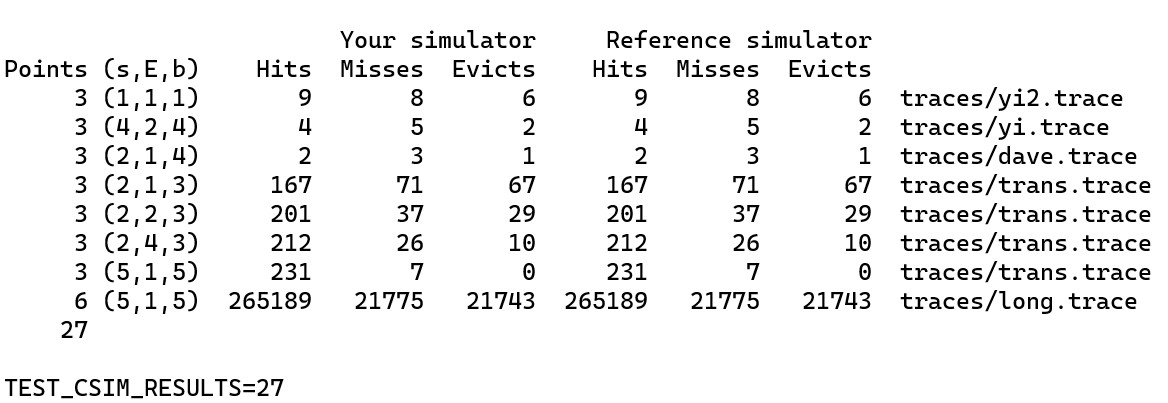
\includegraphics[scale=0.7]{./images/lab1_1.jpg}
		\caption{cache模拟运行结果}
		\label{fig1-1}
	\end{center}
\end{figure}


\newpage
\section{优化矩阵转置}
\subsection{实验目的}
本节实验通过矩阵分块的技术,减少程序对cache的不命中次数,进而优化矩阵转置的性能。本节实验使用的cache为s=5,E=1,b=5,即block offset为5位,set index为5位,一个cache set有一个cache line,也就是直接相联。

\subsection{优化$32\times32$矩阵}
由于block offset为5位,因此一个cache块可以存放32个字节即8个int型数据。对于$32\times32$的矩阵来说,每行的每8个int型数据属于一个cache块,在调入cache时将被一起调入。矩阵和cache set的对应关系如\ref{fig2-1}所示,其中一个矩形代表8个连续的int型数据,标号表示他们映射到的cache set。由该图像可见,将$32\times32$的矩阵划分为$8\times8$的矩阵后,同一个子矩阵内的8行数据属于不同的cache set,当将这8行数据都调入cache后,访问一个$8\times8$的子矩阵内部是不会发生cache冲突的。

实现矩阵转置的最简单的函数如代码\ref{lst:trans}所示。在访问一个$8\times8$的子矩阵时只会在访问初发生强制不命中。在同一列的4个$8\times8$的子矩阵是被映射到同一个cache set中。因此在代码\ref{lst:trans}中,第一层循环遍历A矩阵的一行共32个int型数据,第二层循环遍历B矩阵的一列,这时每访问一个新的$8\times8$的矩阵都会导致8次cache冲突。同时,A和B矩阵在相同位置的元素也被映射到同一个cache set中,这也会导致cache冲突。因此该矩阵转置函数会导致较多的cache不命中。


\begin{figure}[htb]
	\begin{center}
		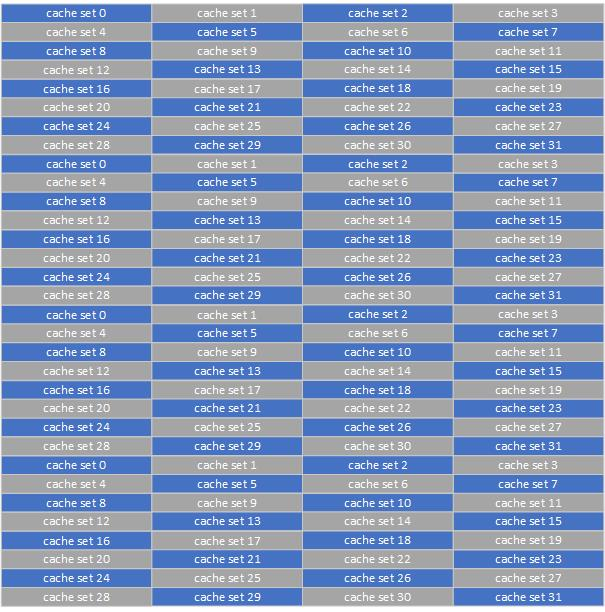
\includegraphics[scale=0.7]{./images/lab2_1.jpg}
		\caption{$32\times32$矩阵和cache set的对应情况}
		\label{fig2-1}
	\end{center}
\end{figure}

\begin{lstlisting}[language=C,caption={简易的矩阵转置函数},label={lst:trans},float=htb]
void trans(int M, int N, int A[N][M], int B[M][N]){
    int i,j,tmp;
    for(i=0;i<N;i++){
        for(j=0;j<M;j++){
            tmp=A[i][j];
            B[j][i]=tmp;
        }
    }
}
\end{lstlisting}





为了适应cache块的大小,使得被调入cache的一个块中的数据被充分利用,防止同一个数据被反复调入cache,我们利用分块技术,将$32\times32$大小的矩阵划分为$8\times8$的矩阵,$8\times8$的矩阵可以被完全调入cache中,除了调入时的强制不命中,在遍历$8\times8$的矩阵的过程中是不会发生cache不命中的。

对于对角线上的$8\times8$矩阵的转置,需要特殊处理。将一个$8\times8$的矩阵被映射到的cache set看作一个集合,$32\times32$的矩阵和cache set的对应关系如\ref{fig2-2}所示,每个矩形表示一个$8\times8$的矩阵,具有相同标号的矩形表示该矩阵对应的cache set为同一个集合。当转置的AB中的矩阵没有位于对角线时,A中子矩阵和B中的子矩阵总是具有不同的标号,因此A的子矩阵和B的子矩阵之间并不会cache冲突。当访问A和B的矩阵中位于对角线上的$8\times8$的矩阵时,每一行的数据属于同一个cache set,且本实验的cache为直接相联,在处理对角线上的矩阵时,当我们读取A[i][i]后,将该值写入到B[i][i]中时,会导致A矩阵中这一行的8个数据所在的cache块被cache驱逐,这会导致较多的冲突不命中。因此,对于A中处于对角线上的$8\times8$矩阵中的每行元素,我们将这一行的元素一次全部读出,放置在8个局部变量组成的缓冲区中,这样在读取矩阵B中的元素时,即使发生冲突导致A中的数据被驱逐,他们将来也不会被访问到。每$8\times8$的子矩阵的转置过程中读取A矩阵会发生8次强制不命中,向B矩阵写入会发生8次强制不命中,$32\times32$的矩阵转置过程中一共会发生256次cache不命中。最终$32\times32$的矩阵的转置过程中cache的运行结果如\ref{fig2-3}所示,发生的cache miss次数为259,其中256次是矩阵转置造成的,3次为函数调用造成的额外开销。

\begin{figure}[htb]
	\begin{center}
		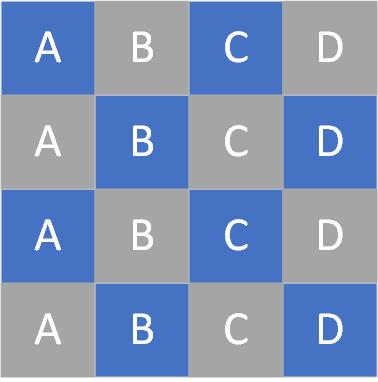
\includegraphics[scale=0.45]{./images/lab2_2.jpg}
		\caption{$32\times32$和cache set的对应情况}
		\label{fig2-2}
	\end{center}
\end{figure}

\begin{figure}[htb]
	\begin{center}
		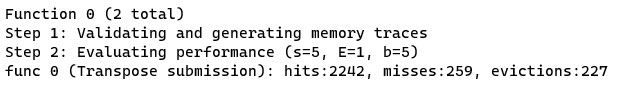
\includegraphics[scale=0.9]{./images/lab2_3.jpg}
		\caption{$32\times32$矩阵转置结果}
		\label{fig2-3}
	\end{center}
\end{figure}

\subsection{优化$64\times64$矩阵}
在$64\times64$矩阵中,我们采用的cache仍然是块大小为32个字节的,因此我们仍希望一次完成同一行的8个数据的转置。当我们对$8\times8$的B矩阵按列访问时,这个矩阵中8行数据与cache set之间的对应关系如\ref{fig2-4}(以第一个$8\times8$矩阵为例)所示。前4个数据和后4个数据分别被映射到同一个cache set中,在访问一列的8个数据的过程中就会产生4次强制不命中和4次冲突不命中,在访问第二列时又会产生8次冲突不命中。这样,B矩阵中的每个数据写入时都会导致一次不命中。

为了防止在一个$8\times8$内部中发生cache冲突,我们在其内部再次划分为$4\times4$的矩阵。不过,cache中一个块为8个int型数据,当我们完成了一个$4\times4$的矩阵的转置后,在这个矩阵之后的$4\times4$的矩阵也被顺带放入了cache中,如果我们此时直接对下一个$4\times4$的矩阵进行转置,那么A和B之中总有一个要将被顺带进入cache的$4\times4$的矩阵从cache中驱逐,之后用到这个矩阵时需要重新调入造成多余的cache不命中。因此,我们应尽可能的利用已经进入cache的块的空间。

将$8\times8$的矩阵划为4个$4\times4$的矩阵,分别记为A[1,1],A[1,2],A[2,1],A[2,2],表示左上,右上,左下和右下的小矩阵。当完成A[1,1]到B[1,1]的转置后,A[1,2]和B[1,2]也已经进入了cache,如果此时直接进行A[1,2]到B[2,1]的转置,B[1,2]会被驱逐出cache,为了利用B[1,2]的空间,我们先将A[1,2]转置放置到B[1,2]中。此时A[1,1]和A[1,2]已经访问完毕,便可以被cache驱逐了。之后我们进行A[2,1]到B[1,2]以及B[1,2]到B[2,1]的转置。首先将B[1,2]的一行读入到一个大小为4的buffer中,接着从A[2,1]中读取一列放入B[1,2]对应的行中,然后把buffer中的数据放入到B[2,1]对应的行中。B[1,2]和B[2,1]中的同一行映射到同一cache set,B[1,2]中的一行的数据通过buffer拷贝,因此这里每一行只会造成一次不命中。对B[1,2]和B[2,1]中的每一行拷贝完成后,再进行A[2,2]到B[2,2]的转置,此时这两个块都位于cache中,不会造成不命中。$8\times8$的矩阵的转置过程如\ref{fig2-5}所示。

\begin{figure}[htb]
	\begin{center}
		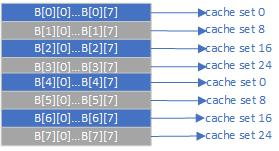
\includegraphics[scale=0.9]{./images/lab2_4.jpg}
		\caption{$64\times64$的矩阵中一个$8\times8$矩阵和cache set的对应情况}
		\label{fig2-4}
	\end{center}
\end{figure}

\begin{figure}[htb]
	\begin{center}
		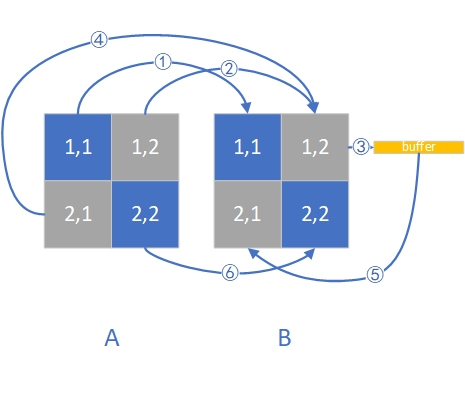
\includegraphics[scale=1]{./images/lab2_5.jpg}
		\caption{$8\times8$矩阵转置示意图}
		\label{fig2-5}
	\end{center}
\end{figure}

和$32\times32$的矩阵类似,A和B矩阵在处理非对角线上的块时彼此之间仍然不会发生cache冲突。但是对于处于对角线上的块时,不仅在$8\times8$矩阵内部会产生cache冲突,A和B矩阵之间也会产生cache冲突。\ref{fig2-5}中的过程中1和2之间,4和5之间以及6的过程中会产生大量的冲突不命中。

这种情况下不能再把B中的空间作为矩阵A的缓存区,为了避免对角线的情况下的冲突不命中,我们把B矩阵中下一个将要进行转置的$8\times8$矩阵作为缓存区\cite{ref1}。此时转置过程的示意图如所示。C[1,1]和C[1,2]表示的是B矩阵中下一轮循环将要用到的$8\times8$矩阵的左上角和右上角的块。为了避免A矩阵中A[1,1],A[1,2]和A[2,1]和A[2,2]之间的冲突,我们首先把A[2,1]和A[2,2]拷贝到C[1,1]和C[1,2]。之后再将A[1,1]和A[1,2]中的内容逐行拷贝到B[1,1]和B[1,2],此时A[2,1]和A[2,2]会被cache驱逐,拷贝完成后,A[1,1]和A[1,2]也会被cache驱逐。

之后将B[1,2]中的数据拷贝到B[2,1]中,这个过程利用buffer逐行拷贝,每将B[1,2]中的一行读出到buffer中后,立即将C[1,1]中的一行拷贝回B[1,2],之后将buffer中的数据拷贝到B[2,1]中,此时B[1,2]中该行会被cache驱逐。最后,将C[2,2]中的数据拷贝到B[2,2]中。

\begin{figure}[htb]
	\begin{center}
		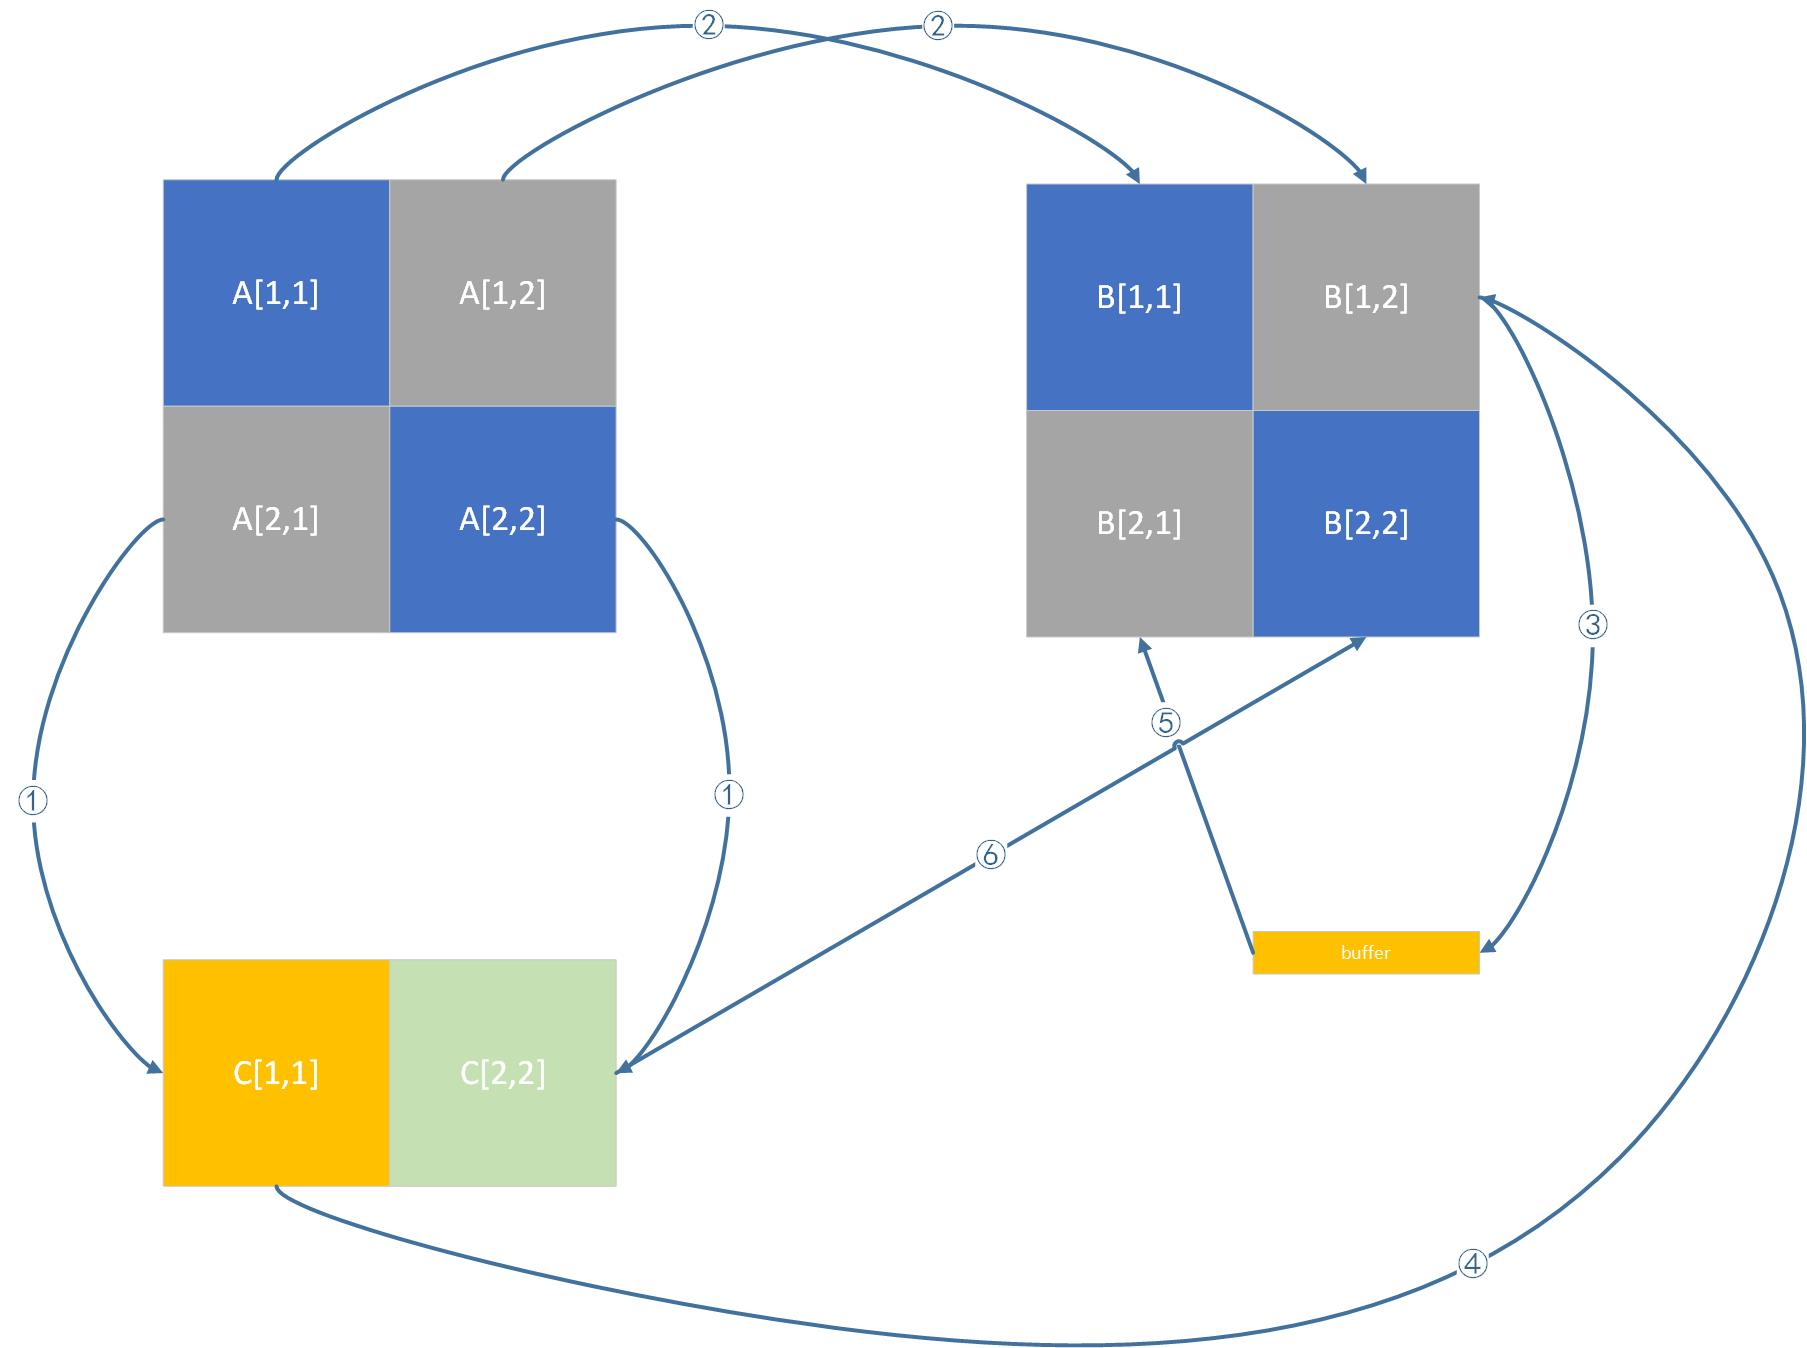
\includegraphics[scale=0.4]{./images/lab2_6.jpg}
		\caption{对角线$8\times8$矩阵转置示意图}
		\label{fig2-6}
	\end{center}
\end{figure}

对角线上的最后一个$8\times8$矩阵没有其他的$8\times8$矩阵作为其缓冲区,因此它只能采取\ref{fig2-5}表示的过程。$64\times64$矩阵转置的运行结果如所示,会产生1046次cache不命中。11+27+11。对于非对角线上和对角线上经过优化的$8\times8$的矩阵转置时会产生16次cache miss,那么$64\times64$会产生1024次cache miss,由于对角线上最后一个$8\times8$的矩阵以及函数调用的开销,会增加22次cache miss。

\begin{figure}[htb]
	\begin{center}
		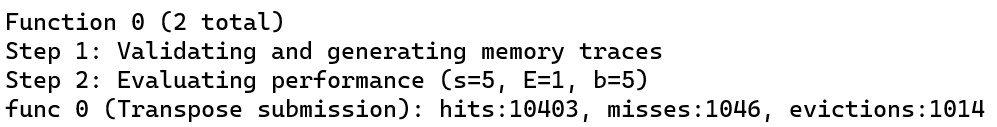
\includegraphics[scale=0.5]{./images/lab2_7.jpg}
		\caption{$64\times64$矩阵转置运行结果}
		\label{fig2-7}
	\end{center}
\end{figure}



\subsection{优化$61\times67$矩阵}
对于$61\times67$的矩阵转置,我们依旧采用矩阵分块的技术。通过尝试分块的大小,将分块设为14可以将不命中次数降为2000次以下。$61\times67$矩阵转置运行结果如\ref{fig2-8}所示。

\begin{figure}[htb]
	\begin{center}
		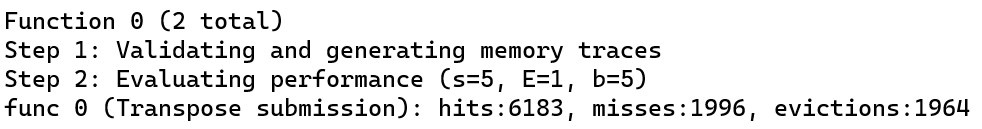
\includegraphics[scale=0.9]{./images/lab2_8.jpg}
		\caption{$61\times67$矩阵转置运行结果}
		\label{fig2-8}
	\end{center}
\end{figure}

\section{总结和建议}

经过本实验,自己对cache是如何实现的有了更深刻的理解,学习了如何利用cache,通过分块技术减少程序的不命中次数从而优化程序性能。

希望本课程对其他章节也设置一些实验,如果只上理论课的话感觉对技术的理解始终比较肤浅。


\newpage
\begin{thebibliography}{99}
  \bibitem{ref1}http://csapp.cs.cmu.edu/3e/cachelab.pdf
  \bibitem{ref2}https://zhuanlan.zhihu.com/p/79058089
  \bibitem{ref3}http://www.cs.cmu.edu/afs/cs/academic/class/15213-f15/www/recitations/rec07.pdf

  \end{thebibliography}
\clearpage

\end{document}
